\subsection{基域变换}

设 N 是 K 的伽罗瓦扩张， \(\Gamma\) 为 N 在 K 上的伽罗瓦群；进一步设 \(N'\) 是 \(K'\) 的伽罗瓦扩张，其伽罗瓦群为 \(\Gamma'\) 。我们将把 K（相应地， \(K'\) ）与其在 N（相应地， \(N'\) ）中的像等同。设 u 为 K 到 \(K'\) 中的同态，v 为 N 到 \(N'\) 中的同态，且 v 在 K 上的限制等于 u（参见

图 1）。设 \(\sigma \in \Gamma'\) ；由于 \(u(\mathbf{K}) \subset \mathbf{K}'\) ， \(\sigma\) 是一个 \(u(\mathbf{K})\) -自同构，作用在 \(\mathbf{N}'\) 上；此外 \(v(\mathbf{N})\) 是 \(u(\mathbf{K})\) 的伽罗瓦扩张，因此 \(\sigma\) 诱导一个 \(u(\mathbf{K})\) -自同构，作用在 \(v(\mathbf{N})\) 上（V，第55页，注记1）。换言之，对每个 \(\sigma \in \Gamma'\) ，存在唯一的元素 \(v^*(\sigma)\) 属于 \(\Gamma\) ，使得

\[
\boldsymbol {v} \circ \boldsymbol {v} ^ {*} (\sigma) = \sigma \circ \boldsymbol {v}.\tag{8}
\]

\pandocbounded{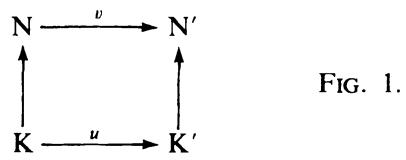
\includegraphics[keepaspectratio]{images/part002_8bfcf433.jpg}}

映射 \(v^*\) 是 \(\operatorname{Gal}(\mathbf{N}' / \mathbf{K}')\) 到 \(\operatorname{Gal}(\mathbf{N} / \mathbf{K})\) 中的同态。对每个 \(x \in \mathbf{N}\) ，映射 \(\sigma \mapsto v^*(\sigma)(x) = v^{-1}(\sigma(v(x)))\) 作为从 \(\Gamma'\) 到离散空间 \(\mathbf{N}\) 的映射是连续的，因此 \(v^*\) 是连续的。

三个特殊情形具有重要意义：

\begin{enumerate}
\def\labelenumi{\alph{enumi})}
\tightlist
\item
  若 F 是 K 的伽罗瓦扩张且 E 是 F 的一个子扩张，我们知道（V，第67页，引理1）F 是 E 的伽罗瓦扩张。让我们将前述内容应用于 N = F， \(K' = E\) ， \(N' = F\) 且 \(v = Id_{F}\) 的情形，则 \(v^{*}\) 仅仅是典范嵌入
\end{enumerate}

\[
j: \operatorname{Gal} (\mathrm{F} / \mathrm{E}) \rightarrow \operatorname{Gal} (\mathrm{F} / \mathrm{K}).
\]

这有时被称为膨胀同态。

\begin{enumerate}
\def\labelenumi{\alph{enumi})}
\setcounter{enumi}{1}
\tightlist
\item
  假设此外 E 在 K 上是伽罗瓦的。让我们将前述内容应用于 N = E， \(K' = K\) ， \(N' = F\) 且 v 是 E 到 F 中的典范嵌入的情形。则 \(v^{*}\) 正是限制同态
\end{enumerate}

\[
\pi : \operatorname{Gal} (\mathrm{F} / \mathrm{K}) \rightarrow \operatorname{Gal} (\mathrm{E} / \mathrm{K}).
\]

我们知道（V，第60页，命题3）， \(\pi\) 是满射，其核为 \(\operatorname{Gal}(\mathrm{F} / \mathrm{E})\) ，并且通过取商，它定义了从 \(\operatorname{Gal}(\mathrm{F} / \mathrm{K}) / \operatorname{Gal}(\mathrm{F} / \mathrm{E})\) 到 \(\operatorname{Gal}(\mathrm{E} / \mathrm{K})\) 上的拓扑群同构（V，第68页，推论4）。

\begin{enumerate}
\def\labelenumi{\alph{enumi})}
\setcounter{enumi}{2}
\tightlist
\item
  假设 \(v^{-1}(\mathbf{K}') = \mathbf{K}\) 且 \(\mathbf{N}' = \mathbf{K}'(v(\mathbf{N}))\) ；让我们证明同态
\end{enumerate}

\[
v ^ {*}: \operatorname{Gal} \left(\mathrm{N} ^ {\prime} / \mathrm{K} ^ {\prime}\right)\rightarrow \operatorname{Gal} (\mathrm{N} / \mathrm{K}),
\]

是一个拓扑群同构，有时称为平移。因为群 \(\operatorname{Gal}(N'/K')\) 是紧致的，群 \(\operatorname{Gal}(N/K)\) 是分离的且 \(v^{*}\) 是连续的；因此只需（《一般拓扑学》，I，第87页，推论2）证明 \(v^{*}\) 是双射。现在，任一元素 \(\sigma\) 若属于 \(v^{*}\) 的核，则它是 \(N'\) 的一个自同构，在 \(K'\) 和 \(v(N)\) 上诱导恒等映射，因此 \(\sigma = \varepsilon\) ，因为 \(\mathrm{N}' = \mathrm{K}'(v(N))\) ；由此可得 \(v^{*}\) 是单射。进一步地， \(v^{*}\) 的像是一个闭子群 \(\Delta\) ，它包含于 \(\operatorname{Gal}(N/K)\) 。

（《一般拓扑学》，I，第81页，同前），且 \(\Delta\) 的不变量域等于 \(v^{-1}(\mathbf{K}') = \mathbf{K}\) ；因此我们有 \(\Delta = \operatorname{Gal}(\mathbf{N}/\mathbf{K})\) （V，第67页，定理4），从而 \(v^{*}\) 是满射。

一般情形可通过复合化归为前述情形。首先我们注意到， \(\mathrm{K}^{\prime}(v(\mathrm{N}))\) 是 \(N^{\prime}\) 中的不变量域，其中 \(\Delta\) 是 \(v^{*}\) 的核；由于 \(\Delta\) 是 \(\operatorname{Gal}(\mathrm{N}^{\prime}/\mathrm{K}^{\prime})\) 的一个正规子群， \(\mathrm{K}^{\prime}(v(\mathrm{N}))\) 是 \(K^{\prime}\) 的一个伽罗瓦扩张（V，第68页，推论4）。因此 \(v^{*}\) 由以下同态复合而成

\[
\operatorname{Gal} \left(\mathrm{N} ^ {\prime} / \mathrm{K} ^ {\prime}\right)\rightarrow \operatorname{Gal} \left(\mathrm{K} ^ {\prime} (v (\mathrm{N})) / \mathrm{K} ^ {\prime}\right) \stackrel {{\psi}} {{\rightarrow}} \operatorname{Gal} \left(\mathrm{N} / v ^ {- 1} \left(\mathrm{K} ^ {\prime}\right)\right) \stackrel {{j}} {{\rightarrow}} \operatorname{Gal} (\mathrm{N} / \mathrm{K});
\]

在此序列中， \(\pi\) 是与三元组 \(\mathbf{K}' \subset \mathbf{K}'(v(\mathbf{N})) \subset \mathbf{N}'\) 相伴的限制同态， \(\psi\) 是与图2中图表中心方块相伴的平移同构， \(j\) 是与三元组 \(\mathbf{K} \subset v^{-1}(\mathbf{K}') \subset \mathbf{N}\) 相伴的膨胀同态。

下一个定理给出了关于平移同构结构的更详细信息。

\[
\begin{array}{c}\mathbf {N} \rightarrow \mathbf {K} ^ {\prime} (v (\mathbf {N})) \rightarrow \mathbf {N} ^ {\prime}\\\uparrow \quad \uparrow\\\mathbf {K} \rightarrow v ^ {- 1} (\mathbf {K} ^ {\prime}) \rightarrow \mathbf {K} ^ {\prime}\end{array}\tag {FIG.2.}
\]

定理 5. --- 设 N' 是由两个子扩张 K' 和 N 生成的 K 的一个扩张。假设N在K上是伽罗瓦扩张，伽罗瓦群为Γ，且K' ∩ N = K。则N'在K'上的扩张是伽罗瓦扩张，并且典范同态φ：K' ⊗K N → N'是一个同构。设σ ∈ Gal(N/K)，并设σ'为在平移同构下与之对应的Gal(N'/K')中的元素；则我们有σ'∘φ = φ∘(Id\_\{K'\} ⊗σ)。

我们有 \(N' = K'(N)\) 且 N 在 K 上是代数且可分的；因此（V，第42页，命题10）， \(N'\) 是 \(K'\) 的一个代数且可分的扩张。由 V 第54页推论4， \(N'\) 是 \(K'\) 的一个拟伽罗瓦扩张。因此 \(N'\) 是 \(K'\) 的伽罗瓦扩张。由上述 c) 可知，映射 \(\sigma \mapsto \sigma | N\) 是一个同态 \(\lambda\) （从 \(\operatorname{Gal}(N'/K')\) 到 \(\operatorname{Gal}(N/K)\) 上）。

我们有 \(N = K'\) {[}N{]} ，因为 N 在 K 上是代数的（V，第18页，推论1），因此 \(\varphi\) 是满射的。如果 \(\sigma\) 属于 \(\operatorname{Gal}(N/K)\) ，我们有

\[
\lambda^ {- 1} (\sigma) \circ \varphi = \varphi \circ \left(\operatorname{Id} _ {\mathrm{K} ^ {\prime}} \otimes \sigma\right).\tag{9}
\]

因此 \(\varphi\) 的核在映射 \(\mathrm{Id}_{\mathbf{K}'} \otimes \sigma\) 下是稳定的，从而具有形式 \(\mathbf{K}' \otimes_{\mathbf{K}} \mathbf{N}_0\) ，其中 \(\mathbf{N}_0 \subset \mathbf{N}\) （V，第63页，推论）。对于 \(x\) （在 \(\mathbf{N}_0\) 中），我们有 \(x = \varphi(1 \otimes x) = 0\) ，因此 \(\mathbf{N}_0 = 0\) ，从而 \(\varphi\) 是单射的。

推论1. --- 设 E' 为 N' 的包含 K' 的子域。存在唯一的包含 K 的 N 的子域 E，使得 E' = K'(E)。我们有 E = E' ∩ N。

令 \(E = E' \cap N\) ，则 \(E' \supset K'(E)\) 。现在令 \(\Gamma = \text{Gal}(N/K)\) ， \(\Delta = \text{Gal}(N/E)\) ，并类似地定义 \(\Gamma'\) 和 \(\Delta'\) 。映射 \(\lambda : \sigma \mapsto \sigma | N\) 是 \(\Gamma'\) 到 \(\Gamma\) 上、也是 \(\Delta'\) 到 \(\Delta\) 上的同构；换言之， \(\Delta'\) 由那些 \(\sigma \in \Gamma'\) 组成，其中 \(\lambda(\sigma)\) 属于 \(\Delta\) 。若 \(\sigma \in \Gamma'\) 保持 \(K'(E)\) 的元素不变，我们有 \(\lambda(\sigma) \in \Delta\) ，从而 \(\sigma \in \Delta'\) 且 \(\sigma\) 保持 \(E'\) 的元素不变；由 V 第68页推论1，我们因此有 \(K'(E) \supset E'\) 。

我们已证明了等式 \(E' = K'(E)\) ，从而 \(\varphi^{-1}(E') = K' \otimes_{K} E\) 。若 F 是包含 K 的 N 的子域，且 \(E' = K'(F)\) ，则同样有 \(\varphi^{-1}(E') = K' \otimes_{K} F\) ，从而 F = E。

推论2. --- 设 N 为 K 的伽罗瓦扩张。假设 N 在 K 上的伽罗瓦群 \(\Gamma\) 是两个闭子群 \(\Gamma_1\) 和 \(\Gamma_2\) 的直积，并记 \(E_i\) 为 \(\Gamma_i\) 的不变量域， \(i = 1, 2\) 。则 \(E_1 \otimes_K E_2\) 到 N 中的典范同态是同构。

我们有 \(E_{1} \cap E_{2} = K\) 且 \(N = K(E_{1} \cup E_{2})\) （由推论6，V，第69页），因此只需应用定理5。

注记. --- 设 K 和 \(K'\) 为两个域，u 为 K 到 \(K'\) 中的同态。设 \(K_s\) （相应地， \(K_s'\) ）为 K（相应地， \(K'\) ）的一个可分闭包（V，第45页，命题14）， \(\Pi\) （相应地， \(\Pi'\) ）为 \(K_s\) 在 K 上（相应地， \(K_s'\) 在 \(K'\) 上）的伽罗瓦群。由于 \(K_s\) 是 K 的一个可分代数扩张，且 K 的扩张（ \(K_s'\) , u）是可分封闭的，因此存在（V，第45页，推论）一个 \(K_s\) 到 \(K_s'\) 中的同态 v，它延拓 u。由 v 我们得到一个连续同态 \(v^*\) （从 \(\Pi'\) 到 \(\Pi\) 中）。设 \(v_1\) 是 u 的另一个延拓；由于 \(K_s\) 是 K 的一个拟伽罗瓦扩张，存在一个元素 \(\sigma_0\) （属于 \(\Pi\) ）使得 \(v_1 = v \circ \sigma_0\) 。我们得出结论 \(v_1^*(\tau) = \sigma_0^{-1} v^*(\tau) \sigma_0\) 对所有 \(\tau \in \Pi\) 成立。

